\section{Ergebnisse aus Tab.~\ref{tab:literatur}}

Das folgende Kapitel fasst die Ergebnisse der systematischen Literaturanalyse zusammen (vgl. Tab.~\ref{tab:literatur}). Dabei werden die in Kap.~\ref{chap:kriterienkatalog} definierten Kriterien auf die identifizierten Publikationen angewendet.

Insgesamt umfasst die Analyse 151 Veröffentlichungen, die in Tab.~\ref{tab:literatur} aufgeführt sind. Abb.~\ref{fig:1-veroeffentlichungen-jahr} zeigt die jährliche Verteilung der Publikationen. Von den insgesamt 151 Arbeiten wurden 58 im Zeitraum von 2020 bis 2025 veröffentlicht, was einem Anteil von ca. 38~\% entspricht, während weitere 55~% der Publikationen in den Jahren 2000 bis 2020 erschienen.

\begin{figure}[htbp]
    \centering
    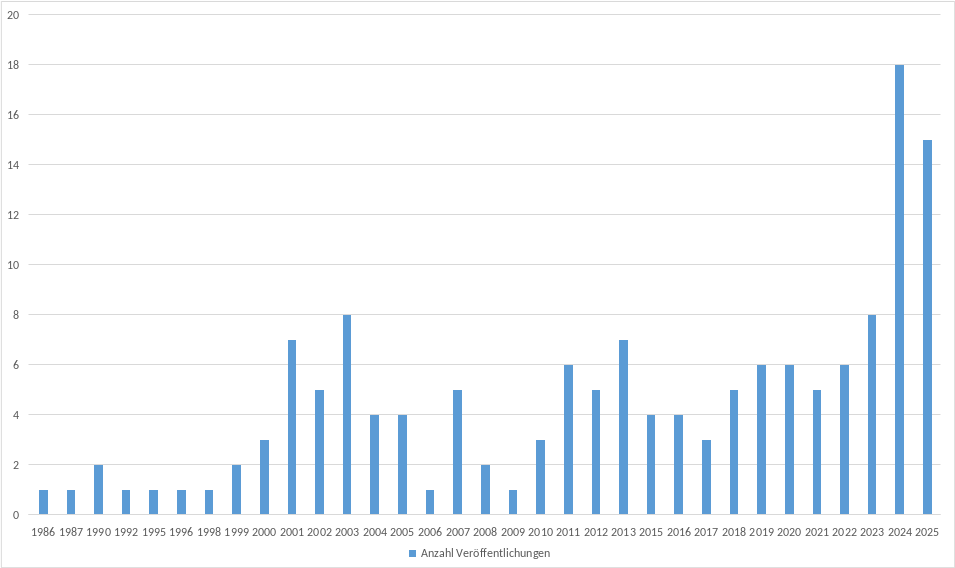
\includegraphics[width=0.90\textwidth]{graphics/1-veroeffentlichungen-jahr.png}
    \caption{Übersicht der Veröffentlichungen pro Jahr}
    \label{fig:1-veroeffentlichungen-jahr}
\end{figure}

Aus Abb.~\ref{fig:2-typ} ist ersichtlich, dass 98~\% der Veröffentlichungen auf Journalartikel (ca. 36~\%) und Konferenzbeiträge (ca. 62~\%) entfallen. Während Journalartikel in Fachzeitschriften mit ausführlicherem Begutachtungsprozess erscheinen, werden Konferenzbeiträge überwiegend in Tagungsbänden veröffentlicht und dienen der schnellen Verbreitung aktueller Forschungsergebnisse. Beide Publikationstypen sind daher für eine Trendanalyse sowie zur Ableitung von Best Practices geeignet.

\begin{figure}[htbp]
    \centering
    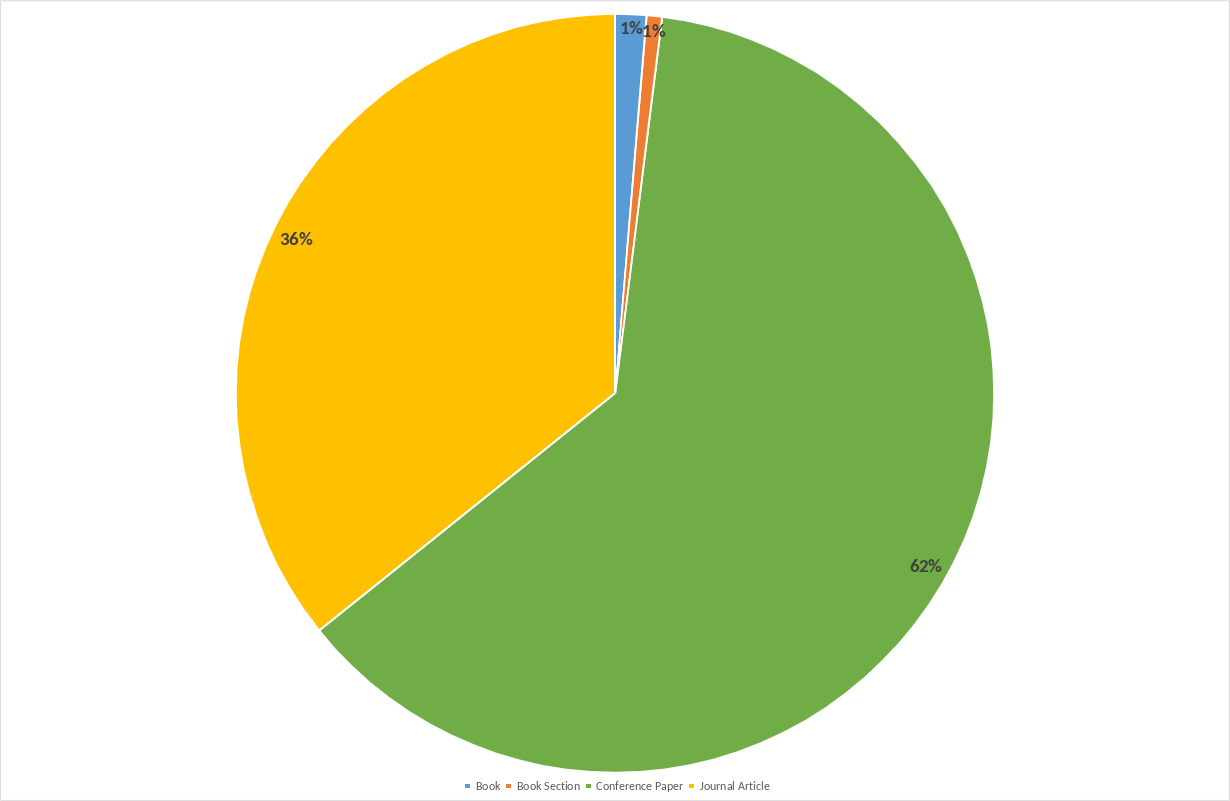
\includegraphics[width=0.90\textwidth]{graphics/2-typ.png}
    \caption{Übersicht des Typs aller Veröffentlichungen}
    \label{fig:2-typ}
\end{figure}

Tab.~\ref{tab:pub-typen} bietet eine Übersicht über die Zeitschriften und Konferenzen, in denen die meisten der untersuchten Publikationen veröffentlicht wurden. Die drei genannten Zeitschriften vereinen 44~\% aller Journalartikel, während die drei aufgeführten Konferenzen rund 22~\% der Konferenzbeiträge ausmachen.

\begin{table}[htbp]
\centering
    \begin{tabularx}{\textwidth}{X c}
        \hline
        \multicolumn{2}{l}{\textbf{Journals}} \\
        \hline
        IEEE Transactions on Education & 10 \\
        Computer Applications in Engineering Education & 7 \\
        Journal on Educational Resources in Computing & 7 \\
        \hline
        \multicolumn{2}{l}{\textbf{Konferenzen}} \\
        \hline
        Workshop on Computer Architecture Education & 8 \\
        ACM Technical Symposium on Computer Science Education & 7 \\
        Annual International Symposium on Computer Architecture & 6 \\
        \hline
    \end{tabularx}
\caption{Übersicht der meistgenutzten Journals und Konferenzen in der Literaturauswahl}
\label{tab:pub-typen}
\end{table}

In Abb.~\ref{fig:3-anzahl-themen} ist ersichtlich, dass die häufigsten Themen der untersuchten Publikationen \enquote{Prozessoren und Architekturen} (44~\%), \enquote{Speicher und Performance} (11~\%) sowie \enquote{Hardware und Logistik} (10~\%) sind. Diese drei Themen umfassen zusammen rund 70~\% aller Publikationen. Dicht darauf folgen die Themen \enquote{Grundlagen und Theorien} sowie \enquote{Programmierung} mit jeweils 9~\% der Arbeiten.


\begin{figure}[htbp]
    \centering
    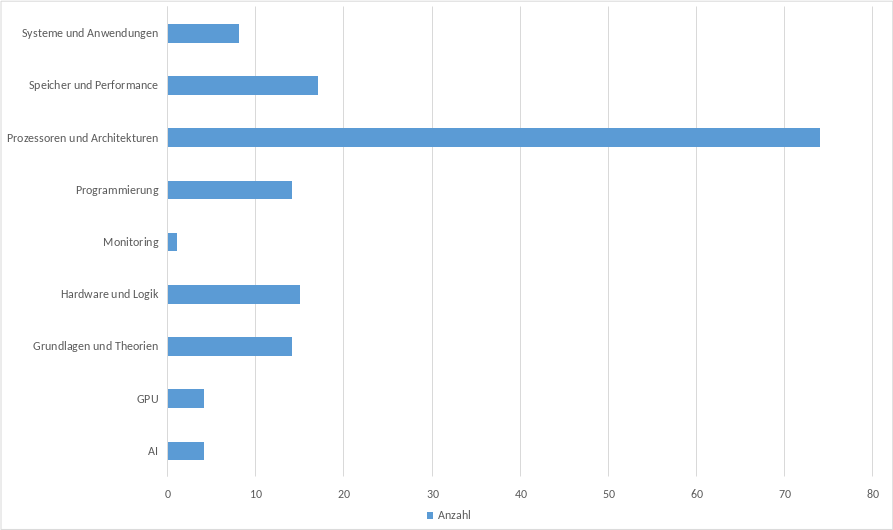
\includegraphics[width=0.90\textwidth]{graphics/3-anzahl-themen.png}
    \caption{Anzahl der Veröffentlichungen pro Thema}
    \label{fig:3-anzahl-themen}
\end{figure}

Eine detaillierte Untersuchung der drei am häufigsten vertretenen Themen ist in Abb.~\ref{fig:4-top3-themen} dargestellt. Die Abbildung zeigt die Verteilung dieser Themen über verschiedene Zeitspannen. Die zugrunde liegenden Werte sind in Tab.~\ref{tab:themen-zeit} aufgeführt.
 
\begin{figure}[htbp]
    \centering
    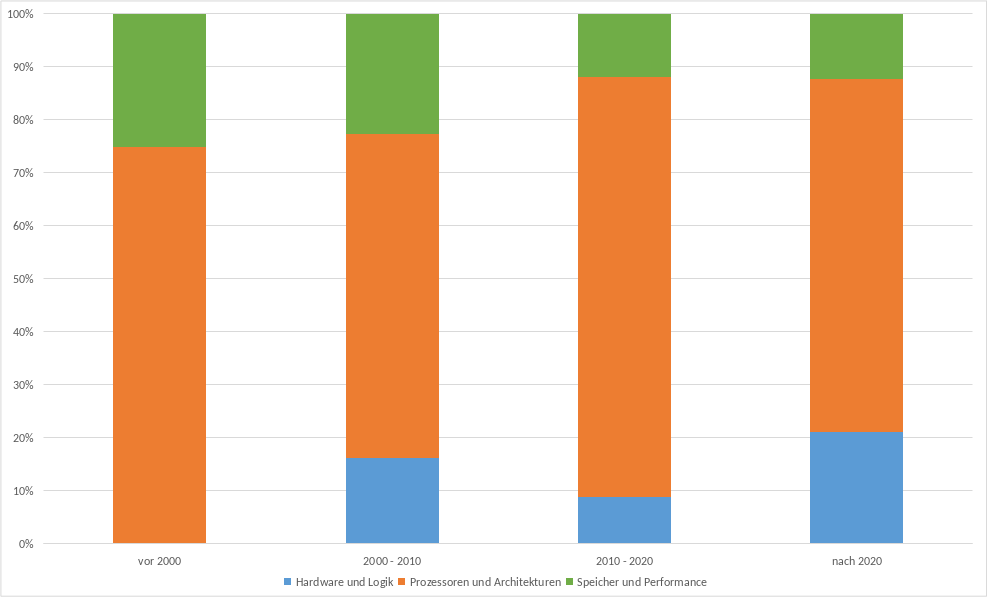
\includegraphics[width=0.90\textwidth]{graphics/4-top3-themen-jahr.png}
    \caption{Jährliche Aufteilung Top 3 Themen}
    \label{fig:4-top3-themen}
\end{figure}

\begin{table}[htbp]
    \centering
    \begin{tabularx}{\textwidth}{lXXX}
        \hline
        \textbf{Zeitraum} & \textbf{Hardware und Logik} & \textbf{Prozessoren und Architekturen} & \textbf{Speicher und Performance} \\
        \hline
        vor 2000      & 0  & 6  & 2 \\
        2000--2010    & 5  & 19 & 7 \\
        2010--2020    & 3  & 27 & 4 \\
        nach 2020     & 7  & 22 & 4 \\
        \hline
    \end{tabularx}
    \caption{Jährliche Aufteilung Top 3 Themen - detailliert}
    \label{tab:themen-zeit}
\end{table}

Für die Themen \enquote{Grundlagen und Theorien} sowie \enquote{Programmierung} zeigt Abb.~\ref{fig:5-top5-themen} die jährliche Verteilung. Die entsprechenden Werte sind in Tab.~\ref{tab:themen-zeit-2} aufgeführt.


\begin{figure}[htbp]
    \centering
    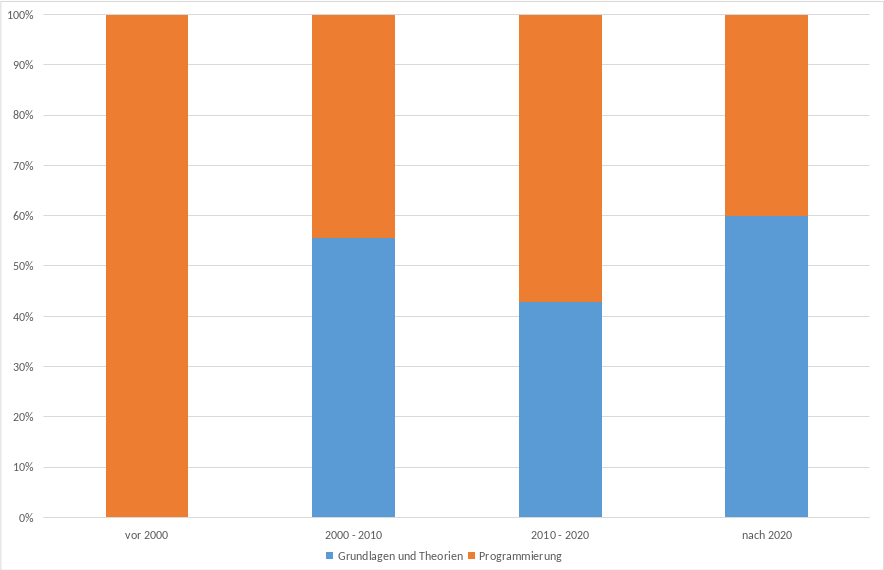
\includegraphics[width=0.90\textwidth]{graphics/5-top5-themen-jahr.png}
    \caption{Jährliche Aufteilung Top 4 und 5 Thema}
    \label{fig:5-top5-themen}
\end{figure}

\begin{table}[htbp]
    \centering
    \tiny
    \begin{tabularx}{\textwidth}{lXX}
        \hline
        \textbf{Zeitraum} & \textbf{Grundlagen und Theorien} & \textbf{Programmierung} \\
        \hline
        vor 2000      & 0 & 2 \\
        2000--2010    & 5 & 4 \\
        2010--2020    & 3 & 4 \\
        nach 2020     & 6 & 4 \\
        \hline
    \end{tabularx}
    \caption{Jährliche Aufteilung Top 4 und 5 Thema - detailliert}
    \label{tab:themen-zeit-2}
\end{table}

Hinsichtlich der Frage, ob die untersuchten Simulatoren spielerische Elemente enthalten, gibt Tab.~\ref{tab:gamification} einen Überblick.

\begin{table}[htbp]
    \centering
    \tiny
    \begin{tabularx}{\textwidth}{lXX}
        \hline
        \textbf{Gamification} & \textbf{Anzahl} & \textbf{\%} \\
        \hline
        Keine Elemente     & 145 & 96\% \\
        Elemente vorhanden & 6   & 4\%  \\
        \hline
        \textbf{Summe}     & 151 & 100\% \\
        \hline
    \end{tabularx}
    \caption{Verteilung der Publikationen in Bezug auf enthaltene Gamification-Elemente}
    \label{tab:gamification}
\end{table}

